\documentclass[12pt]{article}
\usepackage[a4paper, margin=2cm]{geometry}
\usepackage[english]{babel} % To obtain English text with the blindtext package
\usepackage{blindtext}
\usepackage{graphicx} % Required for inserting images
\usepackage{array, multirow} % For extra column formatting
\usepackage{amsmath, amssymb, cancel} %for equation environment
\usepackage{float}
\usepackage{parskip} % For gaps between para
\usepackage{setspace}
\usepackage{pdfpages}
\usepackage{abstract}
\usepackage[export]{adjustbox}
\usepackage{emptypage}
\usepackage{tocloft}
\usepackage[nottoc]{tocbibind}
\usepackage{hyperref, url}
\usepackage[table]{xcolor}
\usepackage{minted}
    \usemintedstyle{monokai}
\usepackage{caption}
    \captionsetup{font=footnotesize,labelfont=bf}
\usepackage{tcolorbox}
    \newtcolorbox{mintedbox}{
        colback=backcolour,
        boxrule=0pt,
        sharp corners,
        width=\linewidth,
        left=0pt, right=0pt,
        top=3pt, bottom=3pt
    }

\cftsetindents{section}{0em}{2em}
\cftsetindents{subsection}{0em}{2em}

\renewcommand\cfttoctitlefont{\hfill\Large\bfseries}
\renewcommand\cftaftertoctitle{\hfill\mbox{}}

\graphicspath{ {./images/} }

\definecolor{blurple}{HTML}{5865F2}
\definecolor{backcolour}{HTML}{272823}

\hypersetup{
    colorlinks=true,
    linkcolor=black,
    urlcolor=black,
    citecolor=blurple,
}

\urlstyle{same}

\renewcommand{\arraystretch}{1.3}

\setcounter{secnumdepth}{5}
\setcounter{tocdepth}{5}
\newcommand\simpleparagraph[1]{%
  \stepcounter{paragraph}\paragraph*{\theparagraph\quad{}#1}}

%%%%%%%%%%%%%%%%%%%%%%%%%%%%%%%%%%%


\title{PHYC20040 Exp.9 Holography}
\author{Joana Adao}
\date{\today}

\begin{document}

\begin{titlepage}
    \begin{center}

        \begin{figure}[ht]
            
\includegraphics[width=\textwidth]{UCDLogo.png}
        \end{figure}
        
        \begin{figure}
            \centerline{
\includegraphics[width=\paperwidth]{UCDBanner.png}}
        \end{figure}

        \vspace{4cm}

        {\LARGE \bfseries PHYC20090 Electronics and Devices}\\
        \vspace{0.75cm}
        {\Large Experiment No.9 Holography}
        
        \vspace{1cm}
    
    {\Large \textbf{24 February 2025}}

    \vspace{2cm}
    
    {\large \textbf{by Joana C.C. Adao (Student No. 23311051)}}\\
    \medskip
    {\large With Ananya L.}

    \end{center}
    
   \clearpage

\end{titlepage}

\setcounter{page}{1}
\tableofcontents
\pagenumbering{roman}

\newpage

\begin{abstract}
\addcontentsline{toc}{section}{Abstract}
\pagenumbering{arabic}

 
\end{abstract}

%%%%%%%%%%%%%%%%%%%%%%%%%%%%%%%%%%%

\vspace{4cm}

\section{Theory} \label{sec:1}

\subsection{Recording and Reconstruction of Holograms}



\subsection{Fourier Transforms}

Consider the reflected waves as seen in Figure \ref{fig:1}. The detailed nature of this "object beam" is dependent on the object's shape and surface
characteristics. Taking a general approach, describe the object beam as a superposition (combination) of plane waves,

\vspace{-2ex}
\begin{gather*}
    \psi_0 (r,t) = A_0 \iint F_0 (k_x,k_y) e^{i(\omega t- k_x x- k_y y - k_z z)} dk_x dk_y 
\end{gather*}

where $(k_x^2 + k_y^2 + k_z^2)^{1/2} = k = \lambda / 2$. Suppose we have permitted this wave $\psi_0$ to interfere with a reference beam given by

\vspace{-2ex}
\begin{gather*}
    \psi_1 (r,t) = A_1 e^{i(\omega t - kz)}
\end{gather*}

and have recorded the resulting intensity pattern on a photographic plate positioned in the plane $z = 0$. The intensity recorded on the plate is then

\vspace{-2ex}
\begin{gather*}
    I(x,y) = \lvert A_1 + A_0 \iint F_0 (k_x,k_y) e^{-i(k_x x + k_y y)} dk_x dk_y \rvert^2
\end{gather*}

Expanding the right-hand side of this equation, we will have terms proportional to $\lvert \psi_0 \rvert^2$, $\lvert \psi_1 \rvert^2$, and $\lvert \psi_0 \psi_1^* \rvert$.

Assuming that the reference beam is much more intense than the object beam (ie. $\lvert \psi_1 \rvert \gg \lvert \psi_0 \rvert$), then the term in $\lvert \psi_0 \rvert^2$ can be ignored,
and the intensity can be approximated as

\vspace{-2ex}
\begin{gather*}
    I (x,y) \approx \lvert A_1 \rvert^2 + A_0 A_1^* \iint F_0 (k_x,k_y) e^{-i(k_xx + k_yy)} dk_x dk_y + A_1 A_0^* \iint F_0 (k_x,k_y) e^{+i(k_xx + k_yy)} dk_x dk_y
\end{gather*}

The transmission function for a developed plate can be expressed as $T(x,y) = 1 - \gamma I(x,y)$ where $\gamma$ is a function of the exposure and
developing processes. Therefore, the hologram's transmission function is

\vspace{-2ex}
\begin{gather*}
    T(x,y) = C_0 - \gamma A_0A_1^* \iint F_0 (k_x,k_y) e^{-i(k_xx+k_yy)} dk_x dk_y - \gamma A_1 A_0^* \iint F_0 (k_x,k_y) e^{+i(k_xx +k_yy)} dk_x dk_y
\end{gather*}

where $C_0$ is a constant. Essentially, the hologram contains both scaled versions of the two-dimensional Fourier tranform of the object beam and its inverse, superimposed on each other.
When this hologram is illuminated with a plane wave life the originall reference beam, another Fourier transformation occurs, which leads to

\vspace{-2ex}
\begin{gather*}
    \psi (r,t) = \iint F(k'_x,k'_y) e^{i(\omega t - k'_xx - k'_yy - k'_zz)} dk'_x dk'_y
\end{gather*}

where, according to Fourier optics,

\vspace{-2ex}
\begin{gather*}
    F(k'_x,k'_y) = \left( \frac{1}{2 \pi} \right)^2 \iint T(x,y) e^{i(k'_xx + k'_yy)} dxdy
\end{gather*}

The three terms that make up $T(x,y)$ obligingly integrate as delta functions (unlike the ignored $\lvert \psi_0 \rvert^2$ term, which would not behave as such), and we find

\vspace{-2ex}
\begin{gather*}
    F(k'_x,k'_y) = - \gamma A_1^* A_0 F_0 (k'_x,k'_y) - \gamma A_1 A_0^* F_0^* (-k'_x, -k'_y) + C_0 \delta (k'_x)\delta(k'_y)
\end{gather*}

As a result, when the hologram is illuminated correctly (as in Figure), the emerging wave consists of three parts: (left) a term that is proportional to the original object beam, effectively
reconstructing the object in all details of amplitude and phase; (centre) a so-called "twin reconstruction" or "twin image", which can be shown to be the original object beam, reflected across the
photographic plate and travelling backwards in time; and (right) an undeflected segment of the reference beam travelling along the z-axis.

\begin{figure}[H]
    \centering
    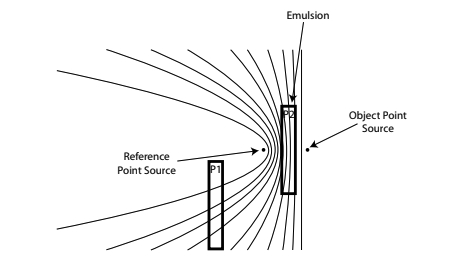
\includegraphics[width=.5\textwidth]{holography1.png}
    \caption{\centering sample caption \protect\cite{princetonholo}}
    \label{fig:1}
\end{figure}

\subsection{Properties of Laser Light in Holography}

\subsubsection{Interference and Diffraction}

\subsubsection{Coherence}


\subsubsection{Monochromaticity}


\subsubsection{Beam Properties: Intensity and Directionality}


\subsection{Amplitude and Phase}


\subsection{Types of Holograms}

\subsubsection{Transmission Holograms}



\subsubsection{Reflection Holograms}





\subsection{Materials and Processing Techniques}

\subsubsection{Photographic Emulsion vs. Photopolymers}


\subsubsection{Chemical Processing}


\subsubsection{Chemical Effects on Hologram Quality}


\subsection{How Shape, Design and Dimension Affect the Hologram}


\subsection{Applications of Holography}


\section{Methodology} \label{sec:2}



\section{Results and Calculations} \label{sec:3}



\newpage

\section{Conclusion} \label{sec:4}



\newpage

%%%%%%%%%%%%%%%%%%%%%%%%%%%%%%%%%%%

\bibliographystyle{IEEEtran}
\bibliography{References} \label{sec:ref}

\vspace{1.5cm}

\listoffigures

\listoftables


\end{document}